\section{Consuntivo a finire}

Nella seguente sezione sono riportati i dati in forma tabellare 
delle ore totali preventivate per la fase RTB rispetto alle ore effettive 
utilizzate dal gruppo SWEnergy.


\subsection{Riepilogo preventivo per la fase RTB}

\begin{table}[H]
	\centering
	\begin{tabular}{l|c|c|c|c|c|c|c}
		\textbf{Nome}         & \textbf{Re} & \textbf{Am} & \textbf{An} & \textbf{Pt} & \textbf{Pr} & \textbf{Ve} & \textbf{Totale ore} \\
		\hline
		Alessandro            & 5           & -           & 5           & 15           & 10           & -           & 35              \\
		Carlo                 & 5           & 5           & 10           & 10           & 5           & -           & 35              \\
		Davide                & 5           & -           & 20          & -           & 5           & 5           & 35              \\
		Giacomo               & 5           & -           & 15          & -           & -           & 5           & 25              \\
		Matteo                & -           & 5           & 10          & -           & 10           & 10           & 35              \\
		Niccolò               & 5           & -           & 10          & 10           & -           & 10           & 35              \\
		\hline
		%\textbf{Ore totali}   & 25          & 10           & 70          & 35           & 30           & 30           & 60              \\
		%\textbf{Costo totale} & 300         & 100         & 1000        & 125         & -           & -           & 1525
	\end{tabular}
	\caption{Re: Responsabile, Am: Amministratore, An: Analista, Pt: Progettista,
		Pr: Programmatore, Ve: Verificatore, Totale: Totale per persona; valori espressi in ore; Costo totale espresso in euro.}
\end{table}

\subsection{Riepilogo consuntivo per la fase RTB}

\begin{table}[H]
	\centering
	\begin{tabular}{l|c|c|c|c|c|c|c}
		\textbf{Nome}         & \textbf{Re} & \textbf{Am} & \textbf{An} & \textbf{Pt} & \textbf{Pr} & \textbf{Ve} & \textbf{Totale ore} \\
		\hline
		Alessandro            & 5           & 5           & 5           & 10           & 10           & -           & 35              \\
		Carlo                 & 10           & 10           & 10           & -           & 5           & -           & 35              \\
		Davide                & 5           & -           & 20          & -           & 5           & 5           & 35              \\
		Giacomo               & 5           & 5           & 5          & 10           & -           & 10           & 35              \\
		Matteo                & -           & 5           & 10          & 5           & 10           & 5           & 35              \\
		Niccolò               & 5           & -           & 10          & 10           & -           & 10           & 35              \\
		\hline
		%\textbf{Ore totali}   & 30          & 25           & 60          & 35          & 30           & 30           & 60              \\
		%\textbf{Costo totale} & 300         & 100         & 750         & 375         & -           & -           & 1525
	\end{tabular}
	\caption{Re: Responsabile, Am: Amministratore, An: Analista, Pt: Progettista,
		Pr: Programmatore, Ve: Verificatore, Totale: Totale per persona; valori espressi in ore; Costo totale espresso in euro.}
\end{table}


\subsection{Periodo RTB}

Di seguito vengono indicate le spese effettive nelle fase RTB del progetto.

\begin{table}[H]
	\centering
	\begin{tabular}{l|c|c|c|c|c|c|c}
		\textbf{Ruolo}         & \textbf{Ore P} & \textbf{Ore E} & \textbf{Diff. ore} & \textbf{Costo orario} & \textbf{Costo P} &\textbf{Costo E} & \textbf{Diff. costo}  \\
		\hline
		Responsabile            & 25                     & 30             & +5                    & 30                   & 750           & 900                     & +150              \\
		Amministratore          & 10                     & 25             & +15                   & 20                   & 200           & 500                     & +300              \\
		Analista                & 70                     & 60             & -10                   & 25                   & 1750           & 1500                   & -250              \\
		Progettista             & 35                     & 35             & 0                     & 25                   & 875           & 875                     & 0              \\
		Programmatore           & 30                     & 30             & 0                     & 15                   & 450           & 450                     & 0              \\
		Verificatore            & 30                     & 30             & 0                     & 15                   & 450           & 450                     & 0              \\
        \hline
        Totale Consuntivo       &                        &                & +10                   &                      &               &                         & +200              \\
		\hline
		%\textbf{Ore totali}   & 10          & 5           & 30          & 15          & -           & -           & 60              \\
		%\textbf{Costo totale} & 300         & 100         & 750         & 375         & -           & -           & 1525
	\end{tabular}
	\caption{Consuntivo periodo RTB, Ore P: Totale Ore preventivate per un singolo ruolo, Ore e: Totale Ore effettive per un singolo ruolo, 
            Diff. ore: Differenza tra ore preventivate e ore effettive, Costo orario: costo orario di un singolo ruolo, Costo P: totale costo preventivato per un singolo ruolo, 
            Costo E: totale costo effettivo per un singolo ruolo,  Diff. costo: Differenza tra costo preventivato e costo effettivo;
            Costo orario: espresso in (\euro/h), Costo P, Costo E, Diff. costo: espressi in (\euro)}  
\end{table}


\subsection{Riepilogo ripartizione percentuale oraria}

\begin{figure}[h]
	\centering
	\begin{tikzpicture}
		\pie[text=legend]{
			14/Responsabile,
			12/Amministratore,
			29/Analista,
			17/Progettista,
			14/Programmatore,
			14/Verificatore
		}
	\end{tikzpicture}
	\caption{Riepilogo ripartizione percentuale oraria}
\end{figure}


\subsection{Riepilogo ruoli per persona}

\begin{figure}[h]
	\centering
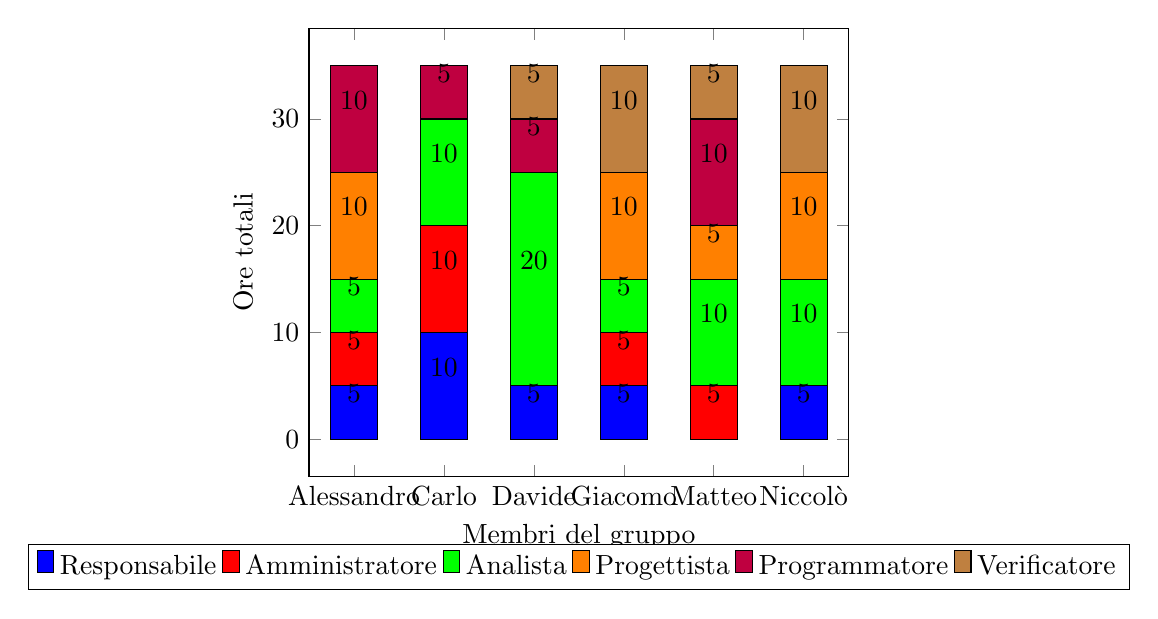
\begin{tikzpicture}
\begin{axis}[
    ybar stacked,
    bar width=0.6cm,
    xlabel={Membri del gruppo},
    ylabel={Ore totali},
    symbolic x coords={Alessandro, Carlo, Davide, Giacomo, Matteo, Niccolò},
    xtick=data,
    legend style={at={(0.5,-0.15)},
    anchor=north,legend columns=-1},
    nodes near coords,
    nodes near coords align={vertical},
]

% Dati per Alessandro
\addplot[fill=blue] coordinates {(Alessandro, 5) (Carlo, 10) (Davide, 5) (Giacomo, 5) (Matteo, 0) (Niccolò, 5)};
\addplot[fill=red] coordinates {(Alessandro, 5) (Carlo, 10) (Davide, 0) (Giacomo, 5) (Matteo, 5) (Niccolò, 0)};
\addplot[fill=green] coordinates {(Alessandro, 5) (Carlo, 10) (Davide, 20) (Giacomo, 5) (Matteo, 10) (Niccolò, 10)};
\addplot[fill=orange] coordinates {(Alessandro, 10) (Carlo, 0) (Davide, 0) (Giacomo, 10) (Matteo, 5) (Niccolò, 10)};
\addplot[fill=purple] coordinates {(Alessandro, 10) (Carlo, 5) (Davide, 5) (Giacomo, 0) (Matteo, 10) (Niccolò, 0)};
\addplot[fill=brown] coordinates {(Alessandro, 0) (Carlo, 0) (Davide, 5) (Giacomo, 10) (Matteo, 5) (Niccolò, 10)};

\legend{Responsabile, Amministratore, Analista, Progettista, Programmatore, Verificatore}

\end{axis}
\end{tikzpicture}

\end{figure}



\subsection{Considerazioni finali}
BLA BLA BLA

